\documentclass[a4paper, openany, oneside]{memoir}
\usepackage[T1]{fontenc}
\usepackage{lmodern}
\usepackage[utf8]{inputenc}
\usepackage[german]{babel}
\usepackage[obeyspaces, hyphens]{url}
\usepackage{graphicx}
\usepackage{listings}
\usepackage{color}
\usepackage{siunitx}
\usepackage[inline]{enumitem}
\usepackage{tabularx}
\usepackage{amsmath}
\usepackage{hyperref}

\graphicspath{{./img/}}


\pretitle{\begin{center}\Huge\bfseries}
\title{User Guide für das Erstellen un Messen von einem JCS}
\posttitle{\par\vskip1em{\normalfont\normalsize Joint-Coordinate-System für sattelförmige Gelenke ausgerichtet nach den Hauptkrümmungsrichtungen nach Halilaj et. al\cite{Halilaj2013}\par\vfill}\end{center}}
\author{Kai Hainke}
\predate{\vfill\begin{center}\large}
\chapterstyle{thatcher}

\DeclareUrlCommand{\dir_path}{\def\UrlLeft{\textrm{»}}\def\UrlRight{\textrm{«}}}

\DeclareUrlCommand{\File_path}{\def\UrlLeft{\textrm{}}\def\UrlRight{\textrm{}}}

\DeclareUrlCommand{\file_ending}{\def\UrlLeft{\textrm{}}\def\UrlRight{\textrm{}}}


\definecolor{dkgreen}{rgb}{0,0.6,0}
\definecolor{gray}{rgb}{0.5,0.5,0.5}
\definecolor{mauve}{rgb}{0.58,0,0.82}
\lstset{frame=tb,
  language=Python,
  aboveskip=3mm,
  belowskip=3mm,
  showstringspaces=false,
  columns=flexible,
  basicstyle={\small\ttfamily},
  numbers=none,
  numberstyle=\tiny\color{gray},
  keywordstyle=\color{blue},
  commentstyle=\color{dkgreen},
  stringstyle=\color{mauve},
  breaklines=true,
  tabsize=3
}



\begin{document}



\maketitle


%\pagebreak
%\dirpath{Documents\BliBla\bludsdus\dssdsd}\linebreak\linebreak
%\url{Documents\BliBla\bludsdus\dssdsd}
%\pagebreak


\chapter{Voraussetzungen}
\section{Tools}
In diesem Guide werden folgende Tools benutzt:
\begin{enumerate}
\item Maya 2014 (insbesondere mit numpy und sklearn)
\item ProKlaue Plugin 0.3.4 
\item R für Plots
\item (zuvor ggf. XROMM Plugin zum Einladen der animierten Szenen)
\end{enumerate}

\section{Verzeichnisstruktur}
Das Basisverzeichnis für diesen Guide ist \\
\dir_path{Documents\ProKlaue\testdaten\achsen}.\\
Darunter sollte wiederum ein Ordner \dir_path{testdaten} mit den Maya-Szenen und ein Ordner \dir_path{ergebnisse} mit den Messergebnissen und den Plots zu finden sein. Im Ordner \dir_path{ergebnisse} sollte pro Tier ein Ordner mit dem Tiernamen angelegt werden und in diesem wiederum ein Ordner für jeden Bodentyp (Beides kleingeschrieben). Auf diese Weise finden sich die Ergebnisse für Alma für den Bodentyp Beton später im Ordner 
\\\dir_path{Documents\ProKlaue\testdaten\achsen\ergebnisse\alma\beton}.\\ 
Die Maya-Szenen im Ordner \dir_path{testdaten} werden wie folgt benannt (auch wenn das recht variabel gehalten werden kann, da diese Namen später spezifiziert werden müssen):\\
\File_path{<Tiername>_ct.mb} für Szenen von Knochen in neutraler Position. \\
\File_path{<Tiername>_<Bodentyp>_<Xerkeys>.mb} für animierte Szenen \\
\File_path{<Tiername>_<Bodentyp>_<Xerkeys>_cs.mb} für animierte Szenen mit JCS \\

\section{Ausgangsdateien}
Es müssen folgende Dateien vorliegen:
\begin{enumerate}
\item 1 Maya-Szene mit Knochen in neutraler Lage für jedes Tier anhand derer das JCS errechnet wird
\item \(x\) animierte Szenen der Knochen, für die die Rotation des entsprechenden JCS gemessen wird, in diesem Fall 1 pro Boden (denkbar wären aber auch mehr oder weniger) 
\item das Python-Skript \File_path{calculateJointCS.py} zum Berechnen des JCS
\item das Python-Skript \File_path{axesToAnimated.py} zum Übertragen des JCS auf die animierten Szenen
\item das Python-Skript \File_path{angles.py} zum Messen der Winkel im JCS.
\item Ggf. das R-Skript \File_path{achsen.R} für Plots aus diesem Guide
\end{enumerate}

\section{Variablen}\label{sec_variables}
Der Nutzer muss außerdem den Wert für folgende Variablen festlegen:
\begin{enumerate}
\item einen Grenzwert zur Bestimmung der Gelenkfläche.\label{th_def} 1 Punkt wird genau dann zur Gelenkfläche gezählt, wenn es ein Punktpaar gibt, für das gilt:
\begin{enumerate}
\item ein Punkt der Paares liegt auf dem distalen Knochen und der andere Punkt auf dem proximalen Knochen und diese beiden Knochen sind Teil des Gelenks,
\item der Abstand zwischen beiden Punkten ist geringer als der festgesetzte Grenzwert.
\end{enumerate}  
\item ein Radius in absoluten Einheiten zur Mittlung der Hauptkrümmungsrichtungen. Ausgehend vom gefundenen Sattelpunkt wird die Fläche innerhalb dieses Radius benutzt, um die Achsen zu berechnen. Dabei werden für die Fläche innerhalb dieses Radius die Hauptkrümmungsrichtungen für jeden Punkt gemittelt. \label{radius_def}
\item absoluter Mess-Fehler für die jeweiligen Gelenke (DIP/PIP links/rechts) \label{error_def}
\item Zeitpunkte des Auffußen (first contact), Abfußen (last contact) und der Hauptstützphase (midstance) für jede animierte Szene bzw. hier jeder Kombination aus Tier und Bodentyp. Jeweils als Nummer des Frames in der animierten Szene. \label{stance_def} 
\end{enumerate}

\chapter{Workflow}

Zunächst wird für jedes Tier eine Maya-Szene mit Knochen in neutraler Position benötigt, um die Achsen für das JCS berechnen zu können. Die Knochen müssen dabei lediglich relativ zueinander neutral liegen, nicht aber global neutral (sie müssen z.Bsp. nicht mit den animierten Szenen eine Ausrichtung oder Bodenebene teilen, wichtig ist lediglich, dass die gleichen Knochen vorliegen). Die Berechnung erfolgt dabei anhand der Hauptkrümmungsrichtungen um den Sattelpunkt des Gelenks, nach einer Methode von Halilaj et al.\cite{Halilaj2013}. Anschließend wird das JCS für jede animierte Szene aus der neutralen Szene übertragen. Abschließend werden über die Animation hinweg für jeden Frame Winkel nach Grood und Suntay\cite{grood1983joint} berechnet.

\section{Erstellen des JCS}
Zunächst öffnet man die Szene mit neutralen Knochenpositionen. Falls die Szene animiert ist navigiert man auf der Timeline zum entsprechenden Frame, indem eine neutrale Position vorliegt. Dann wählt man für jedes Gelenk exakt 3 Knochen aus in der folgenden Reihenfolge (siehe Abbildung \ref{fig:auswahl}):
\begin{enumerate}
\item der distale Knochen des Gelenks
\item der proximale Knochen des Gelenks
\item der linke/rechte Gegenpart zu dem distalen Knochen
\end{enumerate}
Im Beispiel sind das 
\begin{enumerate}
\item Kronbein\char`_rechts:Mesh, 
\item Fesselbein\char`_rechts:Mesh, 
\item Kronbein\char`_links:Mesh.
\end{enumerate} 
Nun passt man folgende Einstellungen im \File_path{calculateJointCS.py} Skript an:

\begin{minipage}[c]{\textwidth}
\begin{lstlisting}
# important settings
threshold = 0.3                 # threshold for defining of the joint surface
radius = 0.9                    # radius to average the principal curvature (from the saddle)
save_dir = "C:/Users/Kai/Documents/ProKlaue/testdaten/achsen/ergebnisse"        # save dir for information file (used for plots later)

# more settings
order = 5                       # order of polynom used to interpolate joint surface
interpolation_order = 3         # order of bivariate spline used to interpolate joint surface in the radius
left = False                    # optional paramter if no third bone is selected to estimate direction to the center of body
axis_used = ["auto"]            # one can specify if to use the minimal or maximal curvature or some automatic setting
\end{lstlisting}
\end{minipage}

Die wichtigsten Einstellungen sind:
\begin{enumerate}
\item der Grenzwert zur Bestimmung der Gelenkfläche, siehe auch Punkt \ref{th_def} in Kapitel \ref{sec_variables}: \lstinline|threshold = 0.3| 
\item der Radius zur Mittlung der Hauptkrümmungsrichtungen um den Sattelpunkt, siehe auch Punkt \ref{radius_def}: \lstinline|radius = 0.9| 
\item das Verzeichnis zum Speichern der Metadaten: \lstinline|save_dir = "C:/Users/Kai/Documents/ProKlaue/testdaten/achsen/ergebnisse"| 
\end{enumerate}
Optionale Einstellungen:
\begin{enumerate}
\item Grad des Polynom-Fits zur Berechnung des Sattelpunktes, Grad der Interpolation durch bivariate Splines in der inneren Fläche  
\item Grad des Splines zur Interpolation der Gelenkfläche bei der Berechnung der Hauptkrümmungsrichtungen
\item manuelle Einstellmöglichkeiten zur Ausrichtung und zur verwendeten Hauptkrümmung (Standardeinstellungen benutzen den 3ten Knochen zur Ausrichtung und eine automatische Auswahl) 
\end{enumerate}


\begin{figure}
\begin{center}
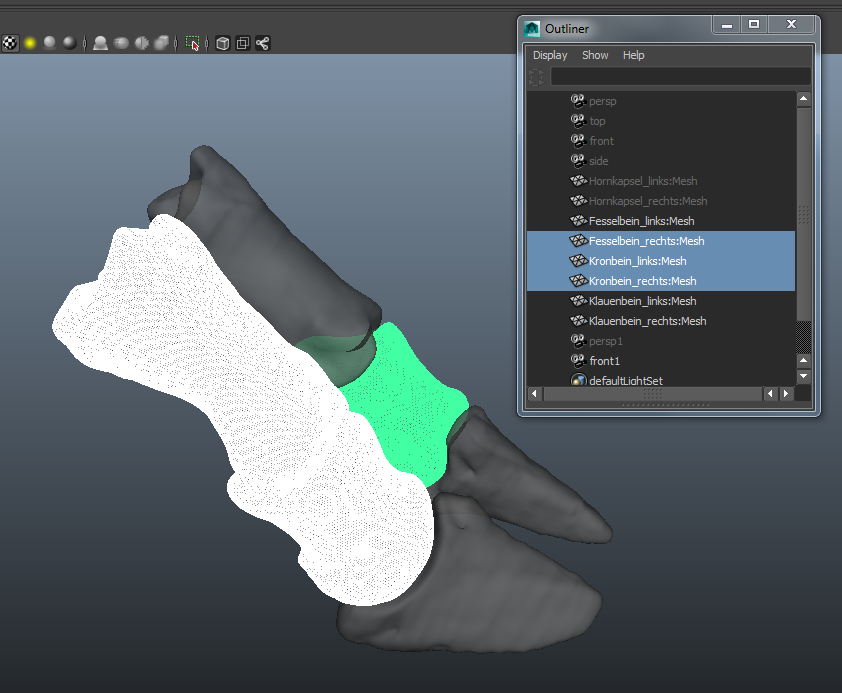
\includegraphics[width = \textwidth, height = 0.4\textheight, keepaspectratio]{img_auswahl}
\caption{Zuerst den distalen, dann den proximalen und dann den Gegenpart auswählen}
\label{fig:auswahl}
\end{center}
\end{figure}

Dann das Script ausführen und man erhält 2 Sattelpunkte mit jeweils 2 Achsen. Dies sind die body-fixed axes der jeweiligen Knochen für das jeweilige Gelenk. Außerdem findet man im vorher festgelegten Verzeichnis die Metadaten für das Koordinatensystem. Diese werden bei den Plots später dafür verwendet, die Werte des Winkels um die floating Axis zu normalisieren. Diese Dateien sollte man in den Ordner des Tieres (bspw. \dir_path{Documents\ProKlaue\testdaten\achsen\ergebnisse\alma} kopieren oder beim Einstellen des Skripts direkt dorthin speichern lassen. (Diese Dateien meint die \File_path{cs-<>-<>.csv} Dateien, in der Regel wird hierbei zuerst der distale und dann der proximale Knochen im Dateinamen stehen). Man sollte die Datei mit den Achsen abspeichern.

\begin{figure}
\begin{center}
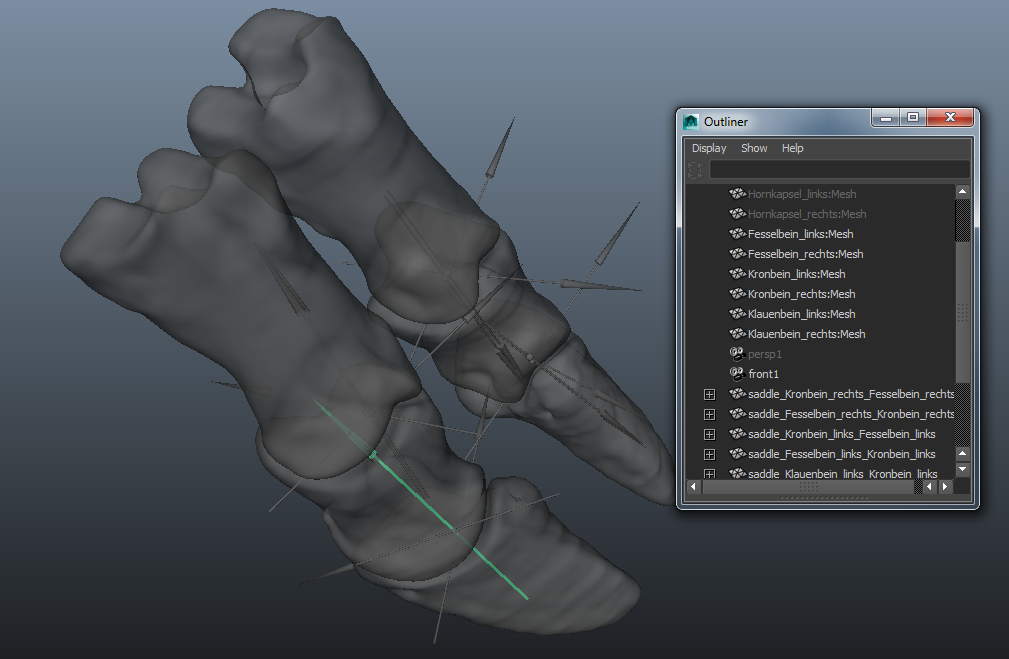
\includegraphics[width = \textwidth, height = 0.4\textheight, keepaspectratio]{img_achsen}
\caption{JCS's nach Ausführen des Skripts (4 mal ausgeführt für 4 JCS's)}
\label{fig:achsen}
\end{center}
\end{figure}

\section{Übertragen des JCS}
Zum Übertragen der Achsen wird das \File_path{axesToAnimated.py} Script verwendet.
Hier sind die folgenden Einstellungen zu treffen:
\begin{enumerate}
\item Grundverzeichnis
\item Namen der Szene in neutraler Position mit den JCS
\item Namen der animierten Szene, in die die Achsen zu übertragen sind
\end{enumerate}

\begin{minipage}[c]{\textwidth}
\begin{lstlisting}
base_dir = "C:/Users/Kai/Documents/ProKlaue/testdaten/achsen/testdaten"           # base dir
scene_animated = "Alma_Karera_8erkeys.mb"     # scene paths relative to base dir
scene_ct = "Alma_ct.mb"
\end{lstlisting}
\end{minipage}

Anschließend für Knochennamen anders als in diesem Projekt standardmäßig verwendet, muss man noch angeben, wie die Knochen in der neutralen Szene und wie in der animierten Szene benannt wurden und welche Achsen zu welchen Knochen gehören sollen.

\begin{minipage}[c]{\textwidth}
\begin{lstlisting}
bones_animated = [u'Hornkapsel_links:Mesh', u'Klauenbein_links:Mesh', u'Kronbein_links:Mesh', u'Fesselbein_links:Mesh',
                  u'Hornkapsel_rechts:Mesh', u'Klauenbein_rechts:Mesh', u'Kronbein_rechts:Mesh', u'Fesselbein_rechts:Mesh']     # bones in the animated scene
bones_ct = [u'Hornkapsel_links:Mesh', u'Klauenbein_links:Mesh', u'Kronbein_links:Mesh', u'Fesselbein_links:Mesh',
            u'Hornkapsel_rechts:Mesh', u'Klauenbein_rechts:Mesh', u'Kronbein_rechts:Mesh', u'Fesselbein_rechts:Mesh']           # in the ct scene

axes = [[], ["saddle_Klauenbein_links_Kronbein_links"],
        ["saddle_Kronbein_links_Klauenbein_links", "saddle_Kronbein_links_Fesselbein_links"],
        ["saddle_Fesselbein_links_Kronbein_links"],
        [], ["saddle_Klauenbein_rechts_Kronbein_rechts"],
        ["saddle_Kronbein_rechts_Klauenbein_rechts", "saddle_Kronbein_rechts_Fesselbein_rechts"],
        ["saddle_Fesselbein_rechts_Kronbein_rechts"]]             # corresponding axes
\end{lstlisting}
\end{minipage}

Dann ausführen und ggf. alle Dialoge bestätigen (zum Speichern, etc.).
\pagebreak
\section{Tracking der Winkel}
Zum Tracken der Winkel wird das \File_path{angles.py} Script verwendet. Dort spezifiziert man wieder folgendes:

\begin{enumerate}
\item Verzeichnis zum Speichern der Dateien
\item zu trackende Frames (hier ein Intervall von \([0,820)\))
\end{enumerate}

\begin{minipage}[c]{\textwidth}
\begin{lstlisting}
base_dir = "C:\\Users\\Kai\\Documents\\ProKlaue\\testdaten\\achsen\\ergebnisse"
frames = range(0, 820) 
\end{lstlisting}
\end{minipage}

Dann die beiden body-fixed Sattelpunkte auswählen (hier \texttt{saddle\char`_<>}). Dabei werden pro Sattelpunkt jeweils die body-fixed axis und die Referenzachse mit ausgewählt. Dabei zuerst den distalen Knochen und dann den proximalen Knochen auswählen (bzw. den Knochen mit der Flexionsachse und dann den ohne). Dabei darauf achten, zusammengehörige Sattel auszuwählen. Also bspw. wählt man zuerst \texttt{saddle\char`_Kronbein\char`_rechts\char`_Fesselbein\char`_rechts} für die Achsen des Kronbeins an dem JCS für das Gelenk zum Fesselbein. Und danach wählt man zusätzlich noch \texttt{saddle\char`_Fesselbein\char`_rechts\char`_Kronbein\char`_rechts} für die Achsen vom Fesselbein aus. Dann das Skript ausführen und es erstellt eine \texttt{rot-<>-<>.csv} Datei mit den Winkelmessungen, diese dann in das jeweilige Verzeichnis des Tieres und des Bodentyps verschieben, also bspw. \dir_path{Documents/ProKlaue/testdaten/achsen/ergebnisse/alma/karera} oder dieses Verzeichnis direkt angeben im Skript (überschreibt ggf. vorhandene Dateien). Diese Dateien können dann bspw. mit R weiter ausgewertet werden. Für dieses Projekt geschieht dies mit dem \File_path{ProKlaue/scripts/JCS_plots_and_data.R} Skript.

\chapter{Hintergrund}
\section{Konvention für die Achsen-Ausrichtung}
Die body-fixed axes werden an den gemittelten Hauptkrümmungsrichtungen ausgerichtet, dabei stehen immer 2 zur Auswahl, die minimale und maximale Hauptkrümmungsrichtung. Standardmäßig werden die Achsen so ausgewählt, dass sie den Konventionen aus Tabelle \ref{tab:ausrichtung_achsen} entsprechen. Die body-fixed axis des distalen Knochen bildet dabei die Flexions-Achse und zeigt daher links und rechts in die selbe Richtung. Für die body-fixed axis des proximalen Knochens ist die Richtung vom linken Knochen entgegen der des rechten Knochen. Dies bewirkt, dass für gegen-gleiche Bewegungen bei bspw. Abduktion/Adduktion gleiche Winkel gemessen werden. Die Referenzachsen werden auf die Position der floating Axis in der neutralen Szene gesetzt. 

\begin{table}[h]
\begin{tabularx}\textwidth{|l|X|X|}
\hline
Position des Knochen & Ausrichtung bfa links & Ausrichtung bfa rechts \\
\hline
distal & rechts \(\rightarrow\) links & rechts \(\rightarrow\) links \\
\hline
proximal & hinten \(\rightarrow\) vorne & vorne \(\rightarrow\) hinten\\ 
\hline
\end{tabularx}
\caption{Ausrichtung der body-fixed axes (bfa)}
\label{tab:ausrichtung_achsen}
\end{table} 

\section{Berechnung der Achsen}
\subsection{Finden von Sattelpunkten auf der Gelenkfläche}
Zur Definition, wann ein Punkt zur Gelenkfläche gezählt wird, siehe Punkt \ref{th_def} in Kapitel \ref{sec_variables}. Zur Berechnung wird hierfür intern ein kd-Baum verwendet. Dann wird die Fläche als Polynom approximiert. Dabei wird Hauptkomponentenanalyse verwendet, um eine Ausrichtung der Fläche zu berechnen, die sich besser eignet, um als Polynom approximiert zu werden. Für die Ableitung des Polynoms wird dann eine Nullstelle gesucht, wo die Hesse-Matrix indefinit, bzw. die Determinante der Hesse-Matrix negativ ist. Also das gängige Verfahren zur Bestimmung von Sattelpunkten auf Polynomflächen.

\subsection{Hauptkrümmungsrichtungen}
Ausgehend von diesem Sattelpunkt wird in einem gewissen Radius das Mesh-Netz der Oberfläche durch ein bivariates Spline interpoliert und für jeden Punkt auf dem Mesh der Shape-Operator wie folgt berechnet. Für ein Polynom \(f(x,y)\) ergibt sich folgende Oberflächendefinition \(P(x,y)=(x,y,f(x,y))\). Die Koeffizienten erster Normalform sind dann:

\begin{align}
E &= 1+\frac{\partial f}{\partial x} \\
F &= \frac{\partial f}{\partial x}\frac{\partial f}{\partial y}  \\
G &= 1+\frac{\partial f}{\partial y} \\
\end{align}   

Die Koeffizienten zweiter Normalform:
\begin{align}
L &= \frac{\partial^2 f}{\partial^2 x}\frac{1}{\sqrt{1+(\frac{\partial f}{\partial x})^2(\frac{\partial f}{\partial x})^2}} \\
M &= \frac{\partial^2 f}{\partial x\partial y}\frac{1}{\sqrt{1+(\frac{\partial f}{\partial x})^2(\frac{\partial f}{\partial x})^2}} \\
N &= \frac{\partial^2 f}{\partial^2 y}\frac{1}{\sqrt{1+(\frac{\partial f}{\partial x})^2(\frac{\partial f}{\partial x})^2}} \\
\end{align}  

Die Normalformen in Matrixdarstellungen sind dann:
\begin{align}
I &=
\begin{pmatrix}
E & F \\
F & G 
\end{pmatrix} \\
II &=
\begin{pmatrix}
L & M \\
M & N 
\end{pmatrix} \\
\end{align}  

Der Shape-Operator ergibt sich dann zu:
\begin{align}
S = I^{-1}II
\end{align} 

Die Eigenvektoren des Shape-Operators sind dann die Hauptkrümmungsrichtungen in Koordinaten des Tangential-Raumes. Die Basis-Vektoren des Tangentialraumes sind:

\begin{align}
v_1 &= \begin{pmatrix}
1 \\
0 \\
\frac{\partial f}{\partial x}
\end{pmatrix} \\
v_2 &= \begin{pmatrix}
0 \\
1 \\
\frac{\partial f}{\partial y}
\end{pmatrix} \\
\end{align} 

Ein Eigenvektor von \((w_1,w_2)\) lässt sich also als folgender Vektor im Beobachtungsraum auffassen:
\begin{align}
\begin{pmatrix}
w_1 \\
w_2 \\
\end{pmatrix} \rightarrow w_1*v_1+w_2*v_2
\end{align} 

Der Eigenvektor mit maximalen Eigenwert gibt die maximale Hauptkrümmungsrichtung vor, der Eigenvektor mit minimalen Eigenwert die minimale Hauptkrümmungsrichtung. Für jeden Punkt in einem vorher festgelegten Radius um den Sattelpunkt werden diese Vektoren (Beobachtungsraum) gemittelt und man erhält die gemittelten Hauptkrümmungsrichtungen, die die Achsen bilden.

\begin{figure}
\begin{center}
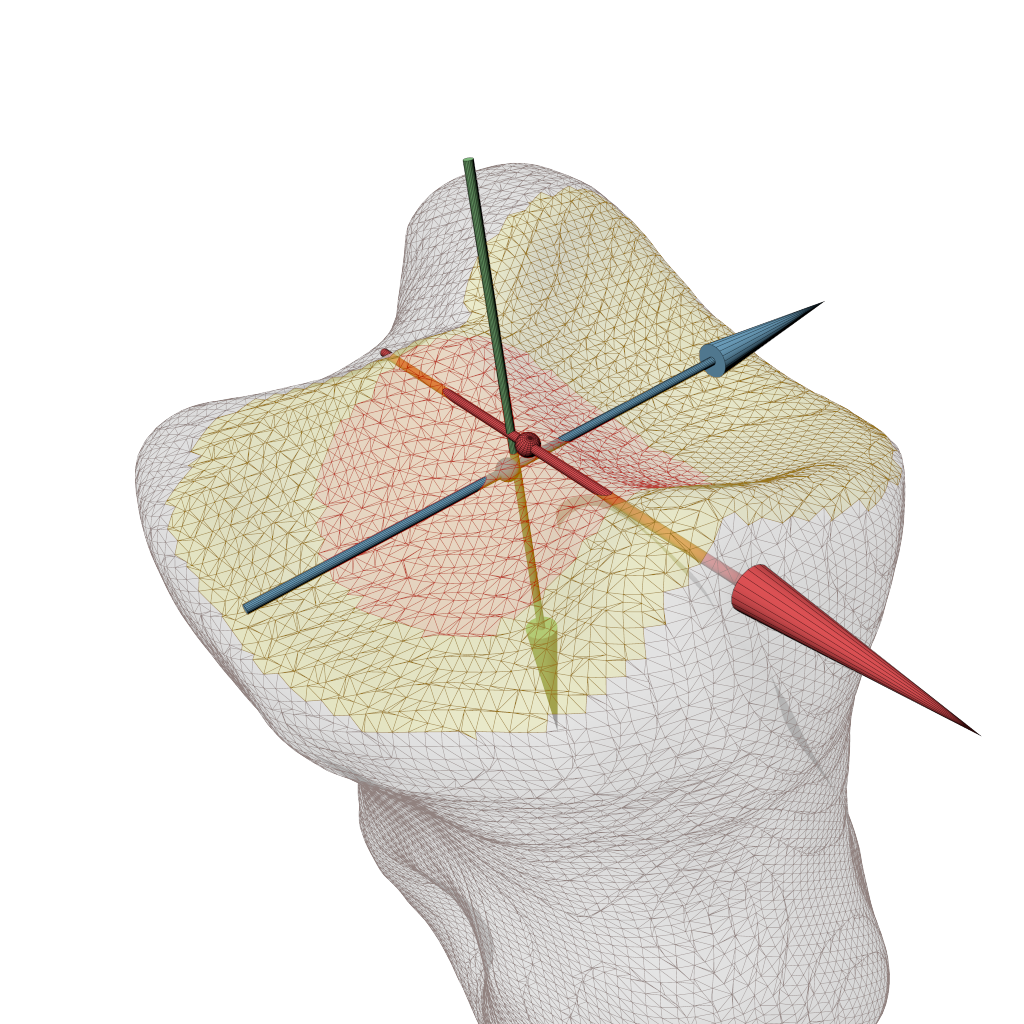
\includegraphics[width = \textwidth, height = 0.4\textheight, keepaspectratio]{vis_1}
\caption{Die gelb markierte Fläche ist die Gelenkfläche, welche zum Auffinden des Sattelpunktes verwendet wird und die rot markierte Fläche gibt die Punkte vor, für die die Hauptkrümmungsrichtungen gemittelt werden. Die rote Achse ist die body-fixed Axis des (unsichtbaren) oberen Knochen und die blaue Achse ist die body-fixed axis des unteren Knochen, also eine der gemittelten Hauptkrümmungsrichtungen aus der roten Fläche (entweder min oder max) }
\label{fig:vis_axes}
\end{center}
\end{figure}


\section{Winkel}
Die Winkelmessungen erfolgen nach Grood und Suntay \cite{grood1983joint}, bedeutet es wird für die beiden body-fixed axes jeweils der Winkel zwischen zugehöriger Referenzachse und floating axis bestimmt und noch der Winkel zwischen den beiden body-fixed axes. Dabei sind erstere beiden einfach zu normieren, indem man die Position der Referenzachsen so wählt, dass sie in einer neutralen Position mit der floating axis zusammenfallen. Dies geschieht, indem man die Referenzachsen in der neutralen Szene auf die Position der floating axis setzt. Letztere Winkelmessung, also der Winkel zwischen den beiden body-fixed axis ist jedoch nicht auf ähnliche Weise zu normieren. Hierfür wird in den Metadaten der Winkel in der neutralen Szene gespeichert und anschließend bei der Datenverarbeitung die gemessenen Winkel auf diesen Wert normiert, so dass bei gleicher Position wie in der neutralen Szene alle Winkel 0 sind. 

\bibliographystyle{abbrv}
\bibliography{lit}
\end{document}